			    A Bitonic Sort\cite{bitonic_ref} is a comparison based parallel sorting algorithm. A random input sequence in first converted into a Bitonic-sequence , which monotonically increases and then decreases thus the name Bitonic.
			    The rotations applied to a Bitonic sequence is also Bitonic.The random input is coversion to Bitonic sequence is achieved with a Bitonic Splitter.\newline
			    Let \[ 
				  S = \langle x_0,x_1,..x_{n-1}\rangle 
				\] be Bitonic sequence such that
				\[
				    x_0 \leq x_1 \leq ... \leq x_{n/2-1} \quad \textrm{and} \quad  x_{n/2} \leq x_{n/2+1} \leq ... \leq x_{n-1}  \quad \textrm{holds}
				\]
			    Consider the following subsequences
				\[
				  S_{1} =  \langle min(x_0,x_{n/2}), min(x_1,x_{n/2+1}),..,min(x_{n/2-1},x_{n-1})\rangle
				\]
				\[
				  S_{2} =  \langle max(x_0,x_{n/2}), max(x_1,x_{n/2+1}),..,max(x_{n/2-1},x_{n-1})\rangle
				\]
			    with the following property.
				\[
				  \forall _{x} \forall _{y}. x \in S_{1}  \wedge  y \in S_{2} \quad x < y
				\]
			    Both $S_{1}$ and $S_{2}$ are Bitonic. A sorted sequence is produced as a result of applying $S_{1}$ and $S_{2}$ recursively. The above procedure is called Bitonic Split. Firstly Bitonic Split is performed the input random sequence which 
			    trasforms any given sequence to a Bitonic sequence which is then fed to the Bitonic Merge Network. The Bitonic Merge converts the splitted sequence to sorted sequence.
			    sequence. A 16 input Bitonic Sorter configuration is shown in the Fig.4. In our case we expand the same configuration to 32 input sorter . The outputs $z_{0}$ to $z_{31}$ are will
			    be connected to the corresponding Functional-Units with respect to the physical address.
				    \begin{figure}[!ht]
					      \includegraphics[width=\linewidth]{BitonicSorter16.png}
					    \caption{A 16 input BitonicNetwork}
				    \end{figure}
			    The arrow indicates a Comparator. The up-down arrow indicates an ascending comparator and the down-to up indicates a descending one. Both the comparator element configurations are shown in Fig.5. An N input Bitonic Network
			    consists of $O(N.log_{2}(N)^{2})$ comparators and has a combinatorial depth of $O(log_{2}(N)^{2})$.
				    \begin{figure}[!ht]
					      \includegraphics[width=\linewidth]{Comparators.png}
					    \caption{Basic 2 x 2 comparator elements of a Bitonic sorter}
				    \end{figure}
			\subsubsection{Bitonic Network as Network Router}
				  The Bitonic-Network is just a sorting network, does not have enough intelligence to act it as a network router in practical cases. Everything works well when all Functional-Units 
				  are ready to send the Data-Packets to its target. But this is not the case most of the times. Many Functional-Units still can be in a state where its outputs are not ready yet,
				  at the same time some of the Functional-Units are ready with the outputs. In this case Bitonic Network can fail in routing the Data-packets to the right destinations because all
				  the not-ready inputs can feed an unknown Target-address. Two solutions were preposed to solve this problem.
				  \subsubsection{Bitonic Network with additional Routers}
					      This is a proposed solution before realizing the Bitonic-Banyan network. In this case the incomplete Target-address problem is sorted out by adding and two extra stages at the input and output of the Bitonic Sorter. At input we add an Address
					      -Resolver module for each comparators. In the architecture an incomplete address is identified by a VALID bit in the data packet (Fig.3). All Functional unit writes a 
					      LOW to the VALID bit of its output packets in every clock cycle unless an packet is ready. In this way the network can interpret the validity of the Data-packet and act accordingly.
					      The Address-Resolver feeds the input of each comparator with a pre-defined hardcoded address according to the position of the comparator. Fig.6 shows a implementation of the
					      Address-Resolver.
					      \begin{figure}[!ht]
							\includegraphics[width=\linewidth]{Address_Resolver.png}
						      \caption{Address resolution}
					      \end{figure}
					      The Address-Resovler is a simple combinatorial multiplexer which switches the address based on the VALID bit of address and is connected to all the N comparators of input.
					      For an N input BitonicNetwork the Hardcoded-Address is obtained by the formula $N -1 + C$ , where C is the position of the the comparator which ranges from 1 to $N$. This ensures the 
					      comparator is fed with an address which is greater that $N -1$, which enables the sorter to work even if some of the inputs are not ready. One more problem that to be resolved
					      still is the output of the network. The sorter will sort the Data-Packets with all the Hardcoded-Addresses in the comes at last but still the actual addresses can
					      be routed into wrong destinations. For eg: If the input has a set of addresses $\{31,X_{1},X_{2},..,X_{31}\}$ (where $X_{i}$ indicates invalid address) which results in the output address set of $\{31,32,33,..,63\}$.
					      The routing is wrong since the 31 is routed to target 0. To resolve this we have to use a stage of routers at the output of the network. The routers have forward and reverse
					      routing path and Data-packet is routed to either forward or reverse path based on the distance to the Target. The distance to each destination is hardcoded in a routing table
					      which enables faster decision making. The configuration is shown in Fig.7. A stall signal is required
					      to stop the network to take new Data-packets until the old ones are delivered to the corresponding target Functional-Units. The worst case time for a packet to reach the target
					      from the router network will be $N / 2$ .In other words in the worst case we have to stall Network fro $N/2$ clock cycles without doing anything useful in that time. The best
					      case would be when all the inputs are valid. Besides the circuit is sequencial and the stall is active in most of the cases there exist another problem which is not efficient. 
					      Also a router element is a complicated state machine which consumes considerable amount of resources when we have 32 instances of the same. This fact 
					      lead us to use a Bitonic-Banyan Network which resolves this invalid address problem in constant time.
					      \begin{figure}[!ht]
							\includegraphics[width=\linewidth]{RouterNetwork.png}
						      \caption{Router Network}
					      \end{figure}
				  \subsubsection{Bitonic-Banyan Network}
					      We utilize the self routing property of a Batcher-Banyan network \cite{batcher_banyan_ref} when the invalid Target-addresses are found at the input. The configuration contains
					      a Bitonic Sorting Network cascaded with a Banyan routing network. As in the case of a Bitonic Network we use the 2 X 2 switching element(comparator) but the connection state of this
					      element is determined by the destination tags of the input, in our case the Target address. A BitonicNetwork can is capable or realizing arbritary permutations of the inputs. 
					      But still the routing is not proper with incomplete Data-packet at the inputs. Here comes the use of Banyan Network which can route the sorted outputs to appropriate
					      Target addresses. As mentined before, special kind of modified switching elements are used which is quite differant from the configuration of normal Bitonic comparators.
					      The switching elements are added with some extra logic to route the larger target address Data-packets to the direction pointed by the arrow. 
					      Fig.6 depicts the switch configuration in different possible scenarios. An 'X' indicates incomplete inputs. This switch basically moves all the X inputs to the bottom of the list.
					      Thus for any input sequence of Data-Packets with $U_{0},U_{1},..,U{r-1}$  are the invalid addresses, the Bitonic network will produce an output sequence of $A_{0},A_{1},..,A_{K},..,U,U,..U$ , where
					      $ K = 32 - r -1$. Fig.7 shows the modified switching element for the Bitonic Network of the SCAD machine. The Normal-switch is an ascending comparator which is shown in Fig.5 and
					      the Modified swich the one which is shown in Fig 6.
					      which handles our situation.
						      \begin{figure}[!ht]
						      \includegraphics[width=\linewidth]{Batcher_Switches.png}
						      \caption{Modified switches for handling incomplete Data-packets in Bitonic Network}
					      \end{figure}
					      \begin{figure}[!ht]
						      \includegraphics[width=\linewidth]{Switching_Element.png}
						      \caption{Swiching element of Bitonic Network}
					      \end{figure}
					      \begin{figure}[!ht]
						      \includegraphics[width=\linewidth]{Banyan_Tree.png}
						      \caption{8 input Banyan network}
					      \end{figure}
					      The next stage is a Banyan Network which takes up the sorted sequences by the BitonicNetwork and route to the proper destination. It is proven \cite{batcher_banyan_ref} that 
					      an Banyan network can completely route a sorted list when the incomplete inputs appear either at high end or low end of the list. We have already moved all the incomplete Data-Packets
					      to the lower end of the sequence with the help of modified switch. An 8 input Banyan Network configuraion is shown in Fig(8). We simply expand the same to 32.
					      The Data-Packets in the Banyan Network is based on the $i^{th}$ bit of the Target-Adress, where $i$ is the stage index. For an $N$ input Banyan Network we have $log_{2}(N)$ 
					      stages and combinatorial circuit depth.A Banyan Newtwork is collision free if the input sequences are sorted ascending
					      thus in our case gurantees the delivery of Data-Packets at proper destination since the Bitonic Network in the previous stage will already produce an acending sequence. In our case 
					      the sequence can also have invalid Data-Packets which is in the tail of the sequence. Different scenarios in handling of incomplete input for a Banyan switch is shown in Fig.9. A 'X'
					      corresponds to incomplete inputs. The valid inputs are the bit position of the stage $i$ of the Target-Address. Beased on this bit the Data-packet is routed up or down.
					      \begin{figure}[!ht]
						      \includegraphics[width=\linewidth]{Banyan_Switches.png}
						      \caption{Modified switches for handling incomplete Data-packets in Banyan Network }
					      \end{figure}
					      It has been proven \cite{sorting_network_on_fpgas} that for $N > 8$ the latency
					      due to combinatorial depth of a Bitonic Network is more that when it is piplelined. So we have implemented 5 stage pipleline for th Bitonic Network and a 5 stage for 
					      the Banyan Network.Altogether for the SCAD machine the synchronous Bitonic-Banyan version of DTN is shown in Fig.10.
					      \begin{figure}[!ht]
						      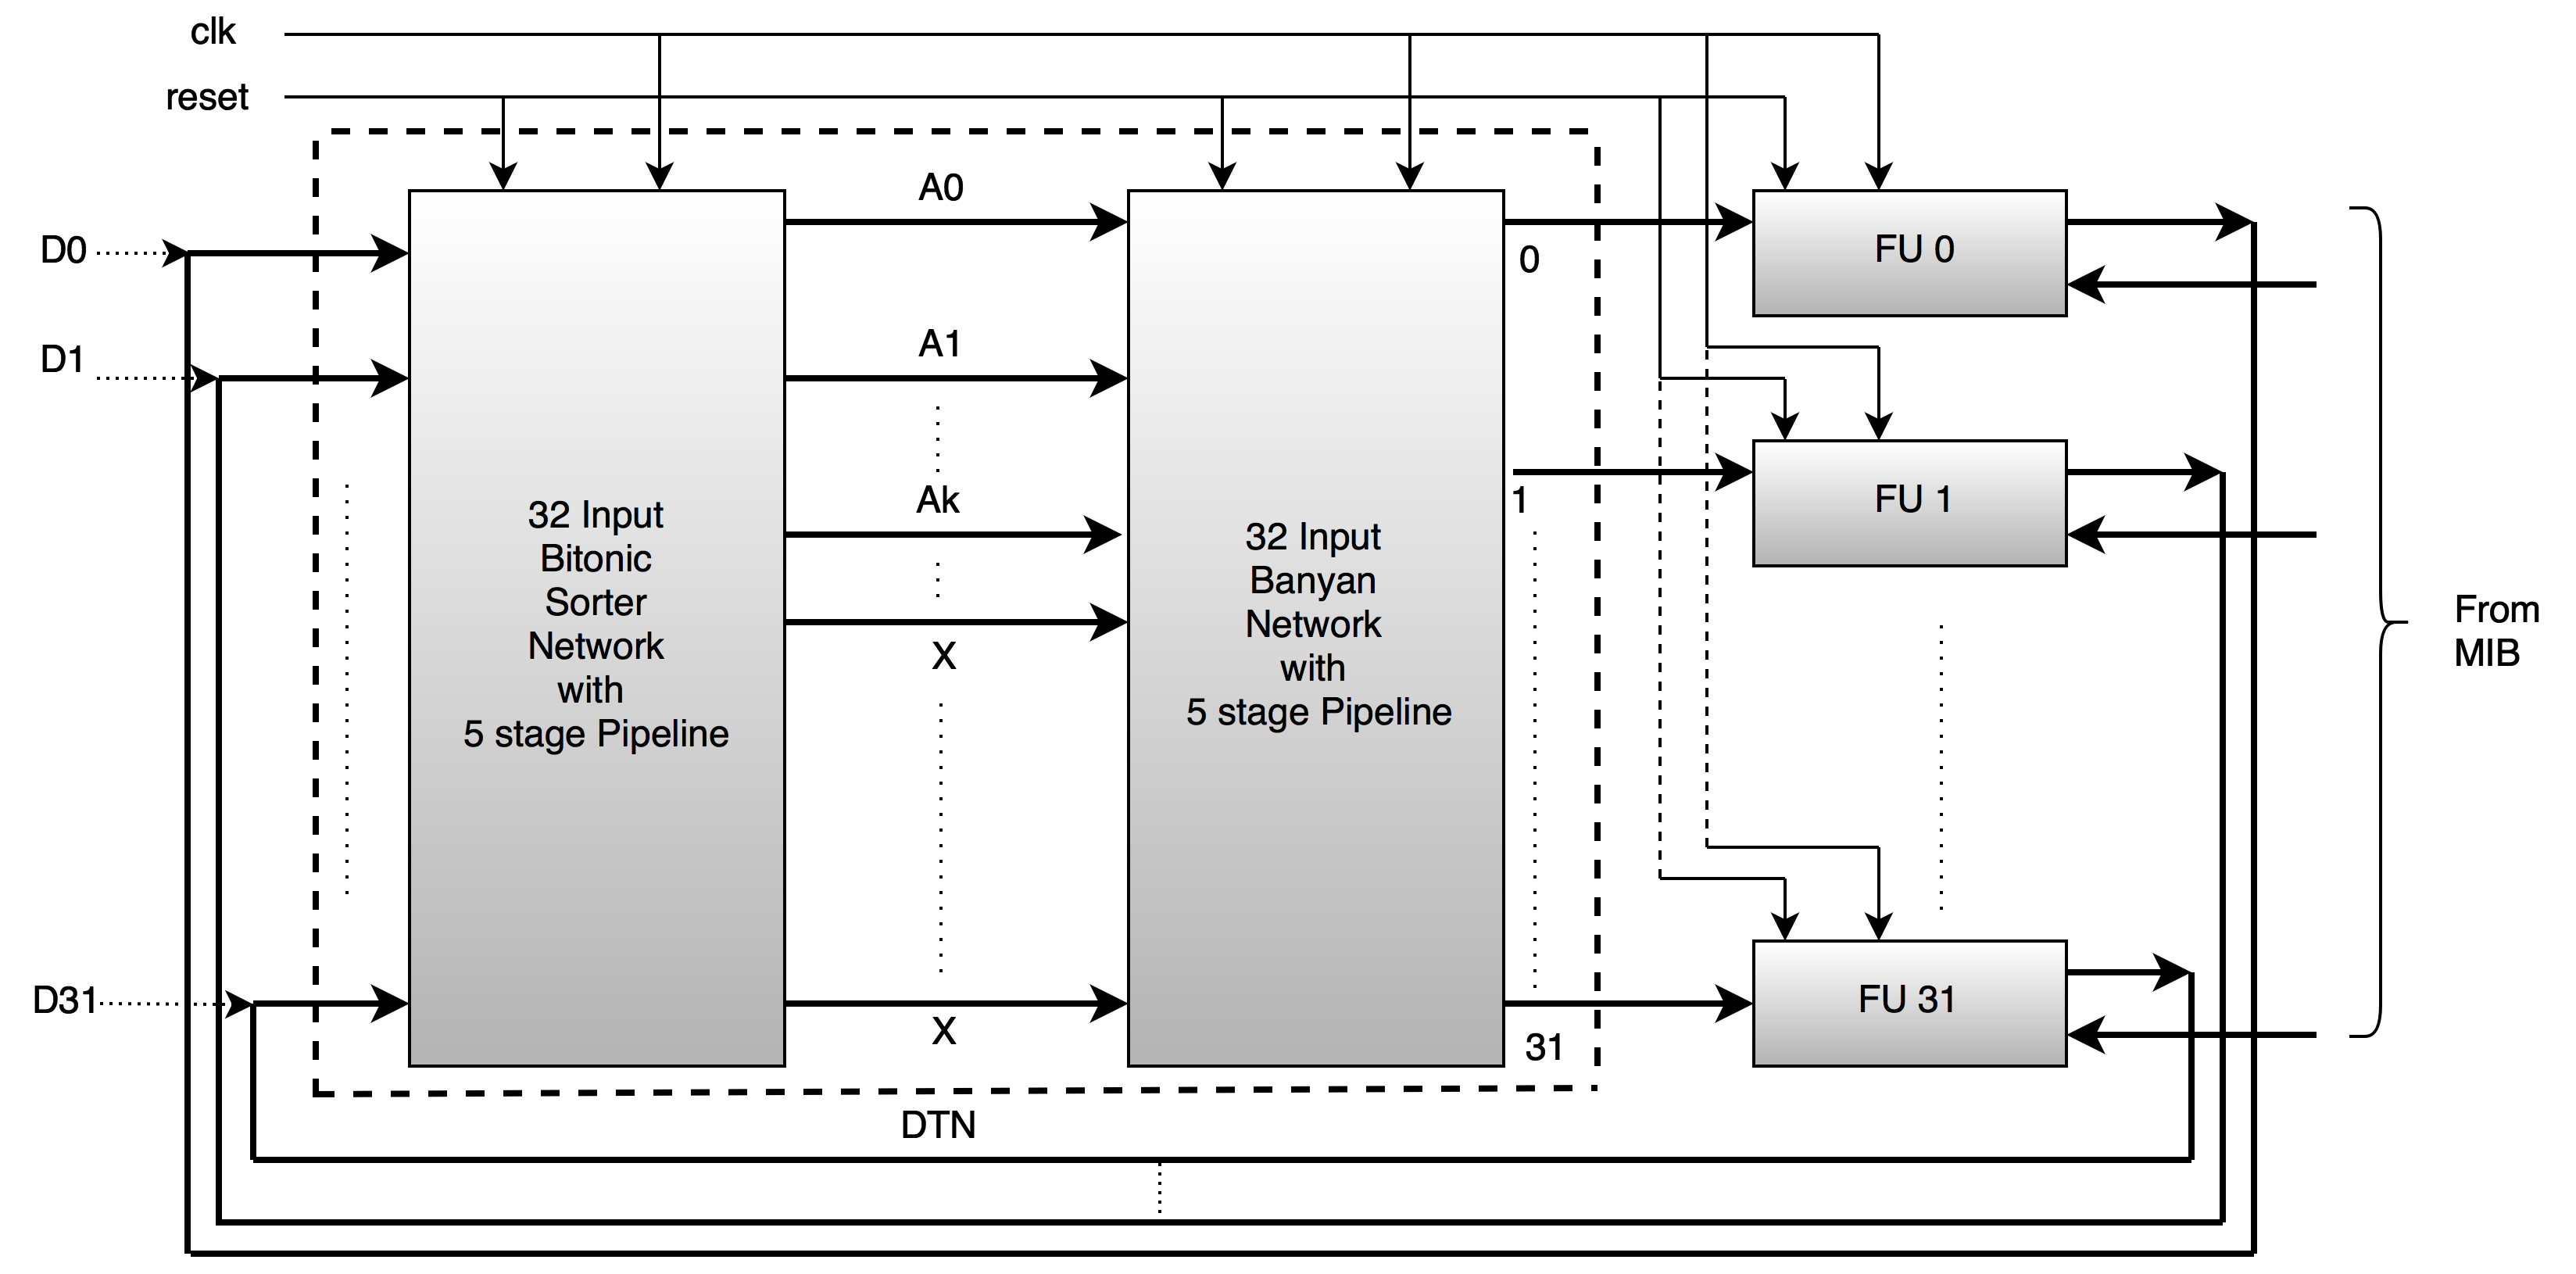
\includegraphics[width=\linewidth]{Batcher_Banyan_Combined.png}
						      \caption{DTN of SCAD machine}
					      \end{figure}

